\documentclass[tikz,border=4pt]{standalone}
\usetikzlibrary{positioning,arrows.meta,calc}
\usepackage[scaled=0.95]{helvet}
\renewcommand{\familydefault}{\sfdefault}
\definecolor{cD}{HTML}{2A78D6}\definecolor{cV}{HTML}{E69F00}\definecolor{cM}{HTML}{009E73}
\definecolor{cK}{HTML}{CC79A7}\definecolor{cL}{HTML}{C0392B}\definecolor{ink}{HTML}{1F2328}
\definecolor{mut}{HTML}{6E7781}\definecolor{pan}{HTML}{F3F5F7}
\tikzset{
  mod/.style={draw=#1, fill=#1!7, rounded corners=4pt, line width=0.9pt},
  ttl/.style={font=\bfseries\footnotesize, text=ink, anchor=north, align=center},
  sub/.style={font=\tiny, text=mut, anchor=north, align=center, text width=#1},
  file/.style={draw=#1, fill=white, rounded corners=2pt, line width=0.6pt, font=\ttfamily\tiny, text=ink,
               inner sep=2pt, minimum height=0.36cm, anchor=west},
  arr/.style={-{Stealth[length=2.3mm]}, line width=0.9pt, color=#1},
  hdr/.style={font=\bfseries\small, text=ink, anchor=west},
  num/.style={circle, draw=ink, line width=0.7pt, font=\bfseries\scriptsize, inner sep=0pt, minimum size=0.42cm},
}
\begin{document}
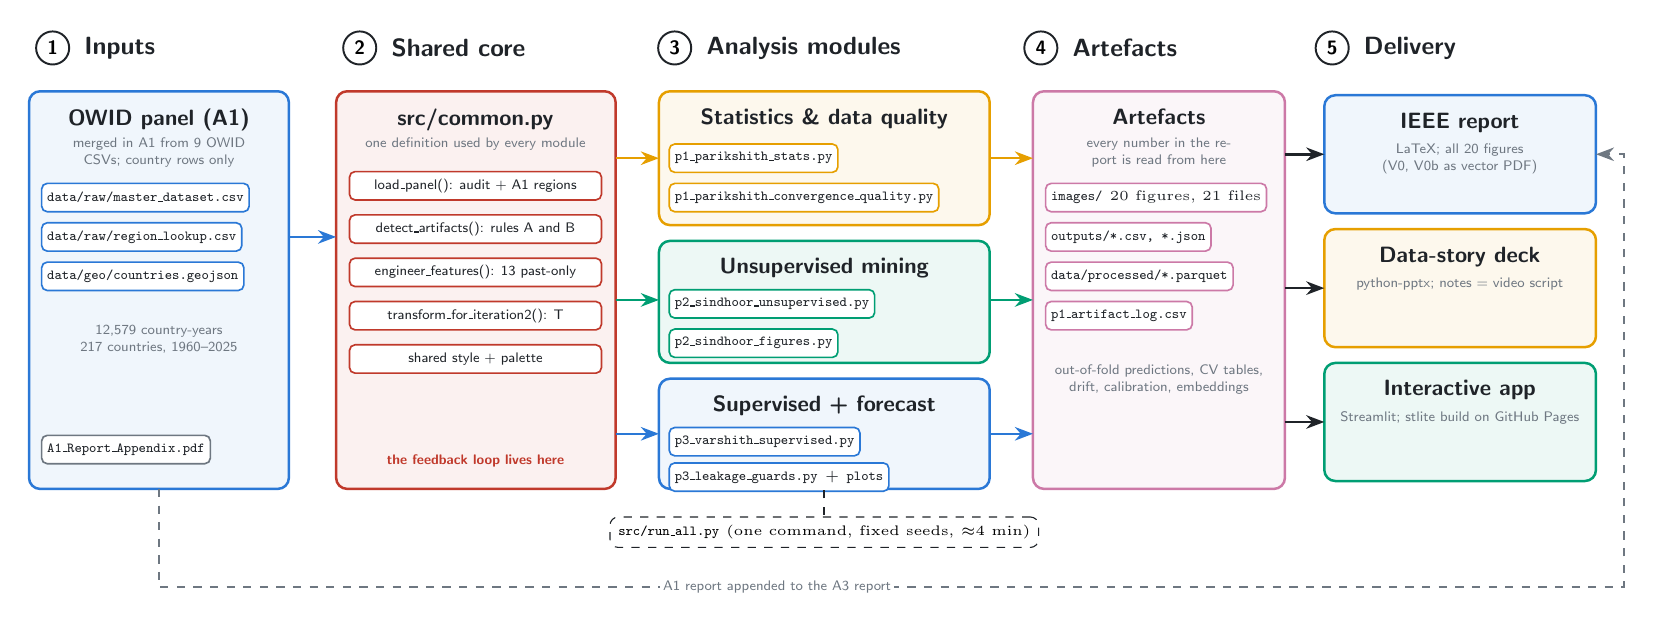
\begin{tikzpicture}[x=1cm,y=1cm]
% headers
\foreach \x/\n/\t in {0.3/1/Inputs, 4.2/2/Shared core, 8.2/3/Analysis modules, 12.85/4/Artefacts, 16.55/5/Delivery}
  {\node[num] at (\x,7.6) {\n}; \node[hdr] at (\x+0.28,7.6) {\t};}

% (1) inputs
\draw[mod=cD] (0,2.0) rectangle (3.3,7.05);
\node[ttl] at (1.65,6.95) {OWID panel (A1)};
\node[sub=3.1cm] at (1.65,6.58) {merged in A1 from 9 OWID CSVs; country rows only};
\node[file=cD] at (0.15,5.7) {data/raw/master\_dataset.csv};
\node[file=cD] at (0.15,5.2) {data/raw/region\_lookup.csv};
\node[file=cD] at (0.15,4.7) {data/geo/countries.geojson};
\node[sub=3.1cm] at (1.65,4.2) {12{,}579 country-years\\217 countries, 1960--2025};
\node[file=mut] at (0.15,2.5) {A1\_Report\_Appendix.pdf};

% (2) shared core
\draw[mod=cL] (3.9,2.0) rectangle (7.45,7.05);
\node[ttl] at (5.67,6.95) {src/common.py};
\node[sub=3.3cm] at (5.67,6.58) {one definition used by every module};
\foreach \t [count=\i from 0] in {load\_panel(): audit + A1 regions, detect\_artifacts(): rules A and B, engineer\_features(): 13 past-only, transform\_for\_iteration2(): T, shared style + palette}
  \node[draw=cL, fill=white, rounded corners=2pt, line width=0.6pt, font=\tiny, text=ink, inner sep=2pt,
        minimum width=3.2cm, minimum height=0.36cm] at (5.67,5.85-\i*0.55) {\t};
\node[font=\tiny\bfseries, text=cL] at (5.67,2.35) {the feedback loop lives here};

% (3) analysis modules
\draw[mod=cV] (8.0,5.35) rectangle (12.2,7.05);
\node[ttl] at (10.1,6.95) {Statistics \& data quality};
\node[file=cV] at (8.12,6.2) {p1\_parikshith\_stats.py};
\node[file=cV] at (8.12,5.7) {p1\_parikshith\_convergence\_quality.py};
\draw[mod=cM] (8.0,3.6) rectangle (12.2,5.15);
\node[ttl] at (10.1,5.05) {Unsupervised mining};
\node[file=cM] at (8.12,4.35) {p2\_sindhoor\_unsupervised.py};
\node[file=cM] at (8.12,3.85) {p2\_sindhoor\_figures.py};
\draw[mod=cD] (8.0,2.0) rectangle (12.2,3.4);
\node[ttl] at (10.1,3.3) {Supervised + forecast};
\node[file=cD] at (8.12,2.6) {p3\_varshith\_supervised.py};
\node[file=cD] at (8.12,2.15) {p3\_leakage\_guards.py \textrm{+} plots};
\node[draw=ink, dashed, rounded corners=3pt, font=\ttfamily\tiny, inner sep=3pt] at (10.1,1.45)
  {src/run\_all.py \textrm{(one command, fixed seeds, $\approx$4 min)}};
\draw[ink, dashed, line width=0.6pt] (10.1,1.67) -- (10.1,2.0);

% (4) artefacts
\draw[mod=cK] (12.75,2.0) rectangle (15.95,7.05);
\node[ttl] at (14.35,6.95) {Artefacts};
\node[sub=3.0cm] at (14.35,6.58) {every number in the report is read from here};
\node[file=cK] at (12.9,5.7) {images/ \textrm{20 figures, 21 files}};
\node[file=cK] at (12.9,5.2) {outputs/*.csv, *.json};
\node[file=cK] at (12.9,4.7) {data/processed/*.parquet};
\node[file=cK] at (12.9,4.2) {p1\_artifact\_log.csv};
\node[sub=3.0cm] at (14.35,3.7) {out-of-fold predictions, CV tables, drift, calibration, embeddings};

% (5) delivery
\foreach \y/\t/\s/\c in {6.25/IEEE report/{LaTeX; all 20 figures (V0, V0b as vector PDF)}/cD, 4.55/Data-story deck/{python-pptx; notes = video script}/cV, 2.85/Interactive app/{Streamlit; stlite build on GitHub Pages}/cM}
{ \draw[mod=\c] (16.45,\y-0.75) rectangle (19.9,\y+0.75);
  \node[ttl] at (18.17,\y+0.65) {\t};
  \node[sub=3.2cm] at (18.17,\y+0.25) {\s}; }

% arrows
\draw[arr=cD] (3.3,5.2) -- (3.9,5.2);
\foreach \y/\c in {6.2/cV, 4.4/cM, 2.7/cD} \draw[arr=\c] (7.45,\y) -- (8.0,\y);
\foreach \y/\c in {6.2/cV, 4.4/cM, 2.7/cD} \draw[arr=\c] (12.2,\y) -- (12.75,\y);
\foreach \y in {6.25, 4.55, 2.85} \draw[arr=ink] (15.95,\y) -- (16.45,\y);
\draw[arr=mut, dashed, line width=0.7pt] (1.65,2.0) -- (1.65,0.75) -- (20.25,0.75) -- (20.25,6.25) -- (19.9,6.25);
\node[font=\tiny, text=mut, fill=white, inner sep=1pt] at (9.5,0.75) {A1 report appended to the A3 report};
\end{tikzpicture}
\end{document}
